\documentclass[conference]{IEEEtran}

% Packages
\usepackage{graphicx}
\usepackage{booktabs}
\usepackage{amsmath}
\usepackage{amssymb}
\usepackage{cite}
\usepackage{url}
\usepackage{listings}
\usepackage{xcolor}
\usepackage{makecell}

% Code listing style
\lstset{
    basicstyle=\ttfamily\footnotesize,
    breaklines=true,
    frame=single,
    language=SQL,
    commentstyle=\color{gray},
    keywordstyle=\color{blue}
}


\lstdefinelanguage{Solidity}{
    keywords={pragma, solidity, contract, function, public, external, view, returns, mapping, struct, event, emit, if, for, while, require, assert, revert, address, bytes32, uint, uint8, uint64, uint256, string, bool, calldata, memory, storage, indexed, indexed, onlyAdmin, onlyPolicyAdmin},
    keywordstyle=\color{teal}\bfseries,
    ndkeywords={function, return, mapping, struct, event, emit, require},
    ndkeywordstyle=\color{brown},
    identifierstyle=\color{black},
    sensitive=false,
    comment=[l]{//},
    morecomment=[s]{/*}{*/},
    commentstyle=\color{gray}\ttfamily,
    stringstyle=\color{red},
    morestring=[b]",
    morestring=[b]'
}


\begin{document}

% Title and authors
\title{Query Performance Analysis of Blockchain-Based Audit Trails for Insurance Access Control}

\author{\IEEEauthorblockN{Anthony Uchenna Eneh $^{1}$, Love Allen Chijioke Ahakonye $^{2}$, Jae Min Lee $^{1}$, Dong-Seong Kim $^{1}$ $^{\ast}$}
	\IEEEauthorblockA{$^{1}$ IT-Convergence Engineering, \textit{Kumoh National Institute of Technology}, Gumi, South Korea \\
		$^{\ast}$ NSLab Co. Ltd., Gumi, South Korea,
		\textit{Kumoh National Institute of Technology}, Gumi, South Korea}
	\IEEEauthorblockA{$^{2}$ ICT Convergence Research Center,
		\textit{Kumoh National of Technology}, Gumi, South Korea}
	{(anthony, loveahakonye, dskim, ljmpaul)}@kumoh.ac.kr}
\maketitle


\begin{abstract}
	Blockchain-based access control offers tamper-proof audit trails for regulatory compliance, but prior work has not quantified query performance, critical for compliance workflows. We present the first comparison of Ethereum event logs against PostgreSQL and MongoDB for audit queries, benchmarking four patterns (by subject, resource, time range, and denials) across 100-10,000 events. Results show blockchain-indexed queries are 6--8$\times$ slower than PostgreSQL, while scan-heavy queries are 35--41$\times$ slower, with significantly higher gas costs, trading latency for immutability. These findings inform hybrid architectures: routing critical decisions to blockchain while delegating routine logs to databases.
\end{abstract}


\begin{IEEEkeywords}
Audit log, Access control, Benchmarking, Blockchain, Ethereum, Insurance
\end{IEEEkeywords}


\section{Introduction}
Auto-insurance claims processing involves sensitive evidence across multiple stakeholders, with regulatory frameworks (GDPR, HIPAA) mandating comprehensive audit trails. Compliance officers must routinely query these trails to answer questions such as ``who accessed this claim file?'' or ``which access requests were denied last month?'' These queries demand low latency and efficient filtering. Traditional centralized systems suffer from tampering vulnerability \cite{centralized_iam}, where malicious insiders can alter or delete logs without detection. ClaimGuard \cite{claimguard_conf}, a blockchain-based ABAC system, addresses this by emitting immutable audit events to the Ethereum blockchain, ensuring tamper-evident records that no single party can unilaterally modify. Prior work demonstrated authorization correctness but \textbf{never quantified audit log queryability}, a critical gap for production deployments where compliance workflows depend on responsive audit queries.

Related work on blockchain audit logging includes BLSQ~\cite{li2024blsq}, which employs Merkle tree optimization for tamper-proof log storage but does not benchmark query latency against databases; BCALS~\cite{bcals2022}, a cloud log management system reporting 55--65~ms insertion latency while focusing on security rather than query patterns; hybrid blockchain-database benchmarks~\cite{hybrid_bcdb2022} analyzing write throughput (100--500~tps) without audit query evaluation; and VeriBench~\cite{veribench2023}, which categorizes verifiable databases but omits Ethereum-to-SQL comparisons. Blockchain ABAC systems such as SmartAccess~\cite{oliveira2022smartaccess} (10--50~tps, 200--800~ms latency) and EHR auditing frameworks~\cite{ullah2024ehr} lack query benchmarks, while G{\"u}rsoy et al.~\cite{gursoy2020eth} report 35--750~ms query latencies for genomic data rather than compliance patterns.

This paper provides the first audit query performance analysis of blockchain-based access control, comparing Ethereum, PostgreSQL 16, and MongoDB 7 across four compliance patterns (100-10K events).

%\section{Related Work}

%Table~\ref{tab:related} compares our work against related approaches. Our work provides the \textbf{first direct comparison} of Ethereum \texttt{eth\_getLogs()} query latency against PostgreSQL and MongoDB for compliance audit patterns---addressing the overlooked dimension of audit \textit{queryability}.

% \begin{table}[t]
% \centering
% \caption{Comparison with Related Works}
% \label{tab:related}
% \scalebox{.8}{
% %\footnotesize
% \begin{tabular}{lccccc}
% \toprule
% Work & \rotatebox{90}{Query Bench} & \rotatebox{90}{DB Comparison} & \rotatebox{90}{Audit Patterns} & \rotatebox{90}{Public Chain} & \rotatebox{90}{Access Control} \\
% \midrule
% BLSQ~\cite{li2024blsq}        & \checkmark &            &            & \checkmark &            \\
% BCALS~\cite{bcals2022}        &            &            & \checkmark &            &            \\
% Hybrid BCDB~\cite{hybrid_bcdb2022} &       & \checkmark &            &            &            \\
% VeriBench~\cite{veribench2023} & \checkmark &           &            &            &            \\
% SmartAccess~\cite{oliveira2022smartaccess} & &          &            & \checkmark & \checkmark \\
% \textbf{This Work}            & \checkmark & \checkmark & \checkmark & \checkmark & \checkmark \\
% \bottomrule
% \end{tabular}}
% \end{table}

\section{System Methodology}

\subsection{ClaimGuard Audit Architecture}

ClaimGuard's audit mechanism consists of an on-chain \texttt{AccessAuditLog} contract that emits indexed events for each access decision, as shown in the Smart contract below.

\begin{lstlisting}[language=Solidity]
event AccessChecked(
    address indexed subject,
    bytes32 indexed resourceIdHash,
    bytes32 indexed actionHash,
    bool allow,
    uint256 ts
);
\end{lstlisting}

The Policy Enforcement Gateway (PEG) calls \texttt{logAccess()} after evaluating policies. Events persist permanently in blockchain transaction logs, queryable via Web3 \texttt{get\_logs()} with indexed filters and block ranges.

\textbf{Query Interface:} Ethereum's event logs support filtering on indexed fields (\texttt{subject}, \texttt{resourceIdHash}, \texttt{actionHash}) and block ranges (\texttt{from\_block}, \texttt{to\_block}). The \texttt{allow} flag is not indexed, so denial queries require full log scanning.

\subsection{Baseline Systems}

\textbf{PostgreSQL 16:} B-tree indexes on \texttt{subject}, \texttt{resource\_id\_hash}, \texttt{timestamp}, and \texttt{allowed}; partial index optimizes denial queries.
\textbf{MongoDB 7:} Indexes on all query fields with schema validation.
Both were deployed in Docker on the same hardware as Ethereum (Hardhat local network).

\subsection{Experimental Design}

\textbf{Event Generation:} 100--10K synthetic events with 200 subjects, 1000 resources, 6 action types, and 80\% allowed / 20\% denied ratio.

\textbf{Query Patterns:} Four compliance-driven patterns: \textit{By Subject} (user audit), \textit{By Resource} (forensic analysis), \textit{Time Range} (periodic reporting), and \textit{All Denials} (security monitoring).

\textbf{Metrics:} Query latency (median, P90, P99 over 10 repetitions) and storage costs, including network overhead.

\textbf{Environment:} Hardhat 3.0, PostgreSQL 16, MongoDB 7 in Docker (Intel i7, 16GB RAM, SSD).

\section{Results and Discussion}
ClaimGuard's blockchain achieves 47 tps with 20.2~ms insertion latency, comparable to SmartAccess (10--50 tps, 200--800~ms) while consuming only 26K gas versus 50-150K. PostgreSQL and MongoDB achieve 62$\times$ and 1000$\times$ higher throughput, respectively.

\subsection{Query Latency Analysis}
Figure~\ref{fig:latency} compares query latency across all systems at 10K events. Indexed queries are 6-8$\times$ slower than in PostgreSQL due to JSON-RPC overhead. Time-range queries are 35$\times$ slower (323.8~ms vs. 9.2~ms) because block scans cannot leverage timestamp indexes. Denial queries are 41$\times$ slower since \texttt{allow} is not indexed on-chain. The performance gap widens with scale: at 10K events, scan-heavy patterns exceed 300~ms, compared to PostgreSQL's sub-10~ms response time. These results confirm that blockchain audit logs are well-suited to low-volume, high-assurance scenarios but require off-chain indexing for larger compliance workloads.

\begin{figure}[!htbp]
	\centering
	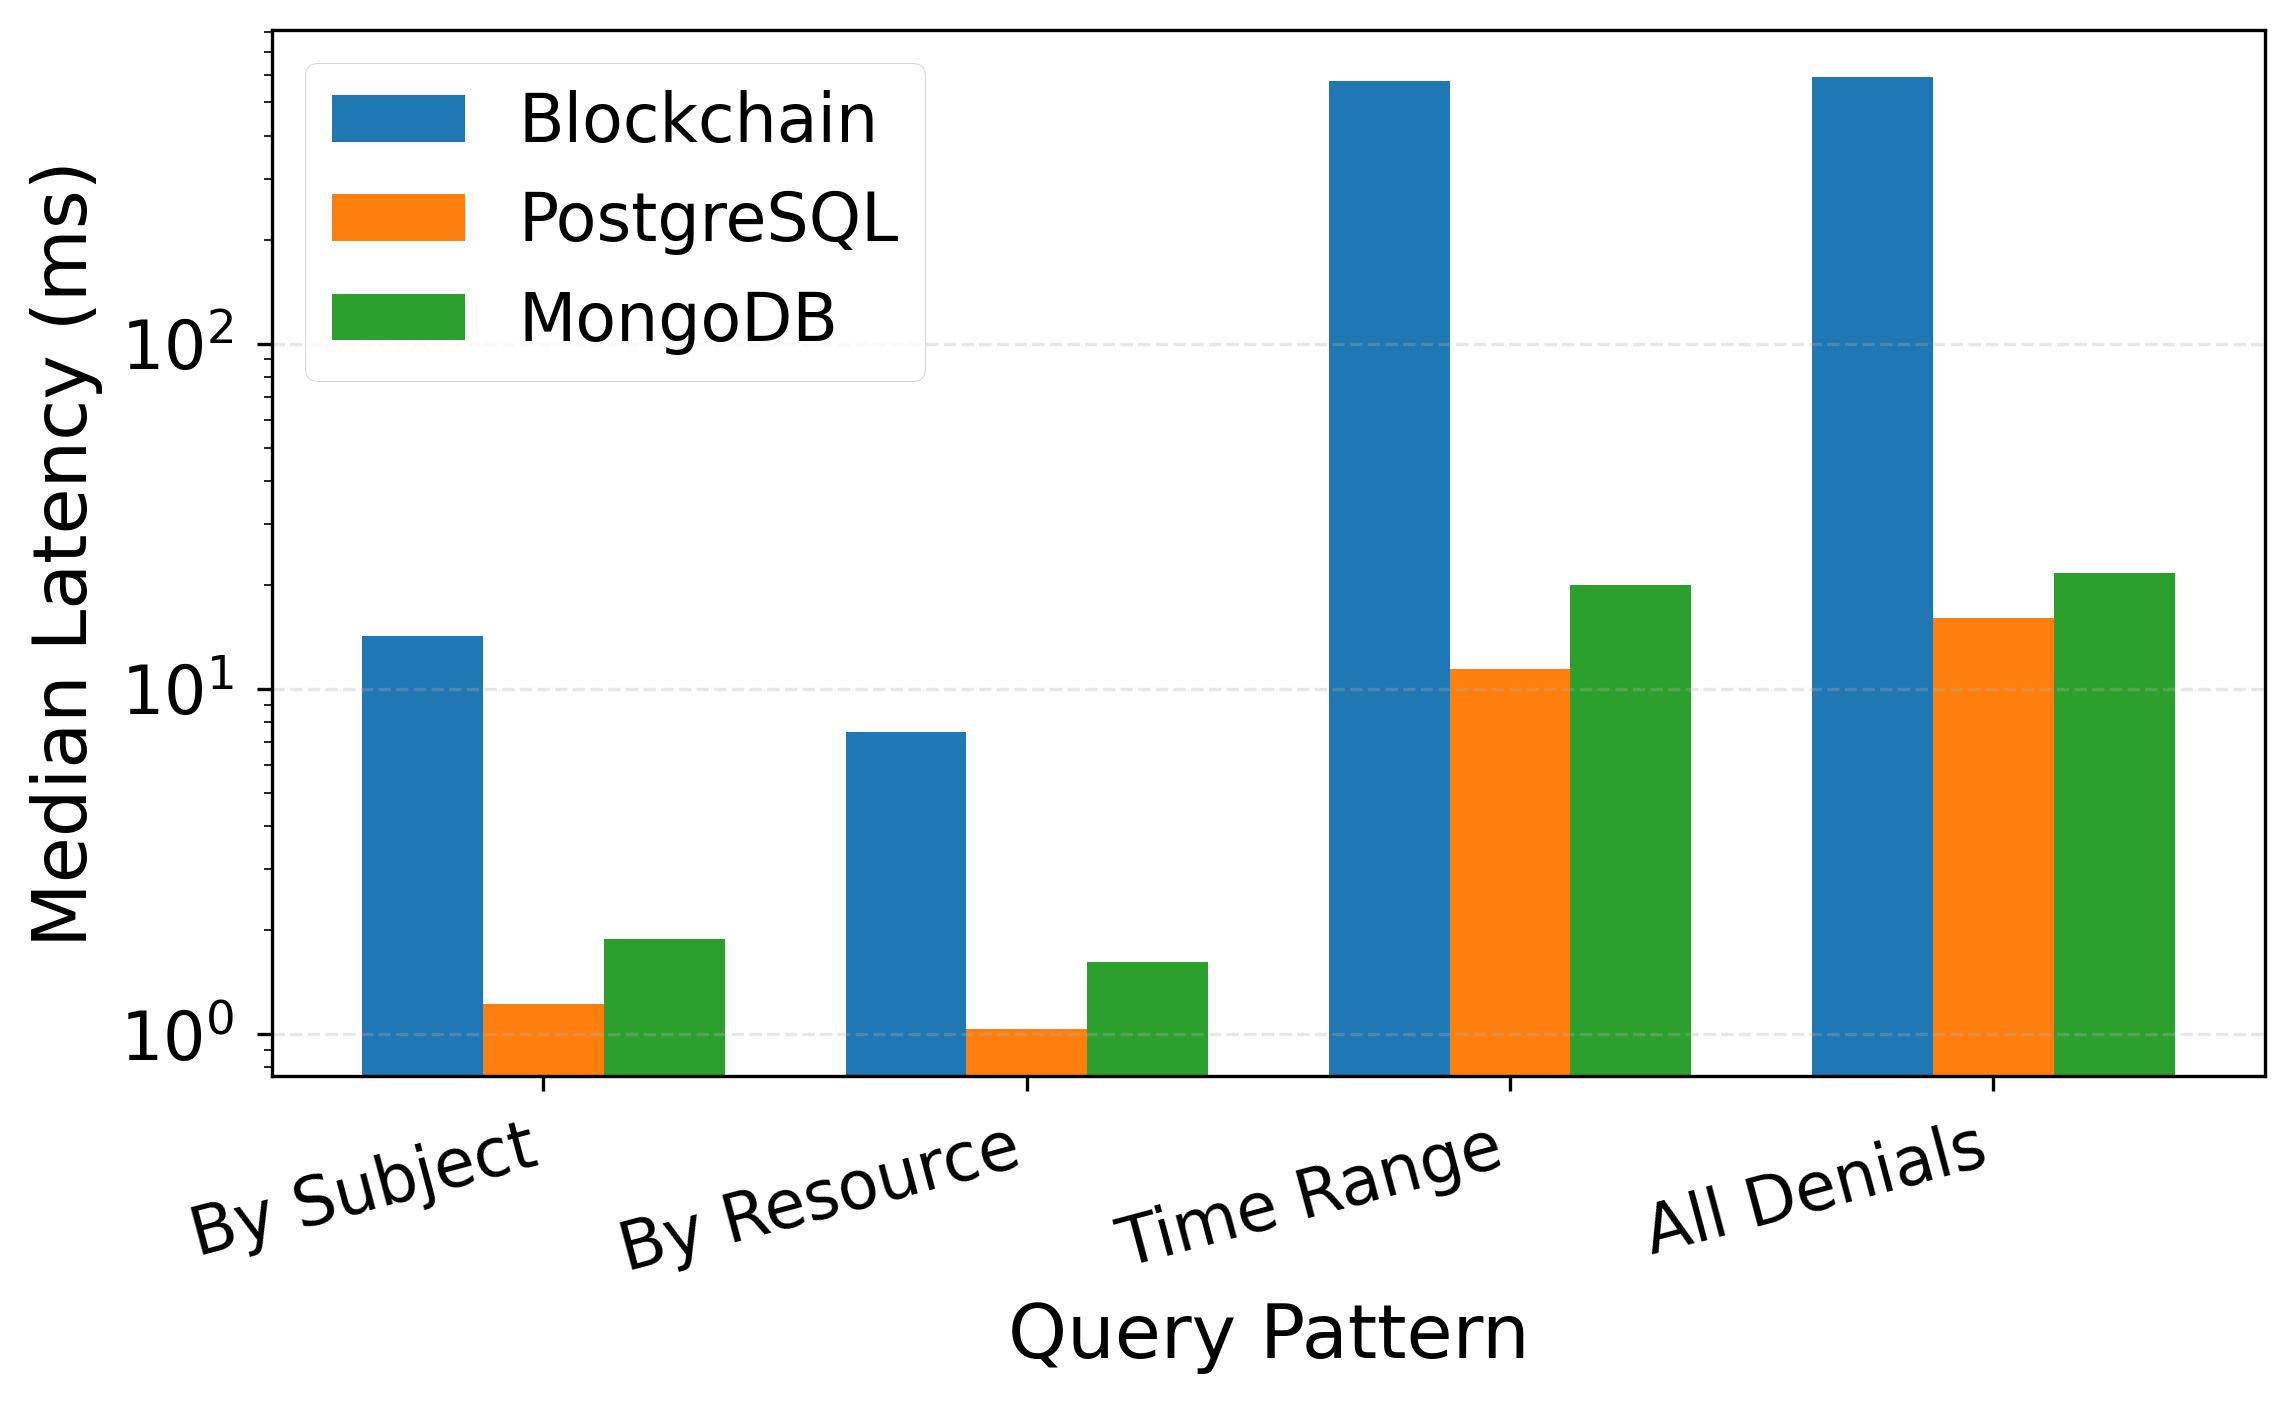
\includegraphics[width=.42\textwidth]{figures/e5_comparison_bar.png}
	\caption{Query latency comparison at 10K events. Indexed queries (By Subject, By Resource) show blockchain 6--8$\times$ slower than PostgreSQL. Scan-heavy queries (Time Range, All Denials) show blockchain 35-41$\times$ slower.}
	\label{fig:latency}
\end{figure}

% \begin{table}[t]
% 	\centering
% 	\caption{Median Query Latency (ms) at 10,000 Events}
% 	\label{tab:latency}
% 	%\scalebox{.8}{
% 		\begin{tabular}{lrrrc}
% 			\toprule
% 			Query Pattern & Blockchain & PostgreSQL & MongoDB & Ratio (BC/PG) \\
% 			\midrule
% 			By Subject    & 9.2        & 1.2        & 3.2     & 7.9$\times$   \\
% 			By Resource   & 6.8        & 1.1        & 2.0     & 6.1$\times$   \\
% 			Time Range    & 323.8      & 9.2        & 19.4    & 35.3$\times$  \\
% 			All Denials   & 335.1      & 8.2        & 15.0    & 40.6$\times$  \\
% 			\bottomrule
% 		\end{tabular}
% \end{table}
%\subsection{Storage Cost Analysis}


%\subsection{Deployment Implications}
Blockchain audit logs are suitable for high-value transactions that require tamper-proof evidence; databases are preferable for high-frequency, cost-sensitive workloads. We recommend a hybrid approach: log critical decisions on-chain while routing routine logs to databases, reducing costs 10--100$\times$.

\subsection{Comparison with Related Works}
Table~\ref{tab:comparison} compares ClaimGuard against related blockchain systems. While prior works focused on write throughput and access control latency, none evaluated audit log \textit{query} performance against traditional databases. Each blockchain event costs $\sim$26K gas (\$0.52 at 10 gwei, \$2K/ETH). PostgreSQL uses $\sim$819 bytes/event; MongoDB $\sim$279 bytes. On-chain storage is orders of magnitude more expensive; 10K events cost $\sim$5,000 on mainnet versus pennies for databases.
\begin{table}[!htbp]
	\centering
	\caption{Performance Comparison with Related Works}
	\label{tab:comparison}
	\scalebox{0.75}{
		\begin{tabular}{lcccc}
			\toprule
			System                                     & \makecell{Write                                                     \\Throughput\\(tps)} & \makecell{Insertion\\Latency\\(ms)} & \makecell{Query\\Latency\\(ms)} & \makecell{Gas Cost\\(per event)} \\
			\midrule
			SmartAccess~\cite{oliveira2022smartaccess} & 10--50             & 200--800       & --        & 50--150K          \\
			Hybrid BCDB~\cite{hybrid_bcdb2022}         & 100--500$^\dagger$ & --             & --        & --                \\
			G{\"u}rsoy et al.~\cite{gursoy2020eth}     & --                 & 400$^\ddagger$ & 35--750   & --                \\
			\midrule
			\textbf{This work}                   & 47                 & 20.2           & 6.8--335  & 26K               \\
			% \textbf{ClaimGuard (PG)}                   & 2,900              & 1.7            & 1.1--9.2  & --                \\
			% \textbf{ClaimGuard (Mongo)}                & 47,000             & 1.0            & 2.0--19.4 & --                \\
			% \bottomrule
			% \multicolumn{5}{l}{\footnotesize $^\dagger$BFT consensus; $^\ddagger$1000 entries; BC=Blockchain, PG=PostgreSQL} \\
		\end{tabular}}
\end{table}

\section{Conclusion}
We present the first quantitative analysis of query performance on blockchain audit logs. Blockchain-indexed queries are 6--8$\times$ slower than PostgreSQL; scan-heavy queries are 35- 41$\times$ slower, with gas costs orders of magnitude higher. These findings support hybrid architectures, routing critical decisions to blockchain while delegating routine logs to databases. Future work includes Layer~2 deployment and off-chain indexing.


\section*{Acknowledgment}
This work was partly supported by the Innovative Human Resource Development for Local Intellectualization program through the IITP grant funded by the Korea government (MSIT) (IITP-2026-RS-2020-II201612, 25\%), by the Priority Research Centers Program through the NRF funded by the MEST (2018R1A6A1A03024003, 25\%), and by the MSIT, Korea, under the ITRC support program (IITP-2026-RS-2024-00438430, 25\%) and by the Basic Science Research Program through the National Research Foundation of Korea(NRF) funded by the Ministry of Education (RS-2026-25431637, 25\%).

\bibliographystyle{IEEEtran}
\bibliography{references}

\end{document}
